%%%%%%%%%%%%%%%%%%%%%%%%%%%%%%%%%%%%%%%%%
% Short Sectioned Assignment
% LaTeX Template
% Version 1.0 (5/5/12)
%
% This template has been downloaded from:
% http://www.LaTeXTemplates.com
%
% Original author:
% Frits Wenneker (http://www.howtotex.com)
%
% License:
% CC BY-NC-SA 3.0 (http://creativecommons.org/licenses/by-nc-sa/3.0/)
%
%%%%%%%%%%%%%%%%%%%%%%%%%%%%%%%%%%%%%%%%%

%----------------------------------------------------------------------------------------
%	PACKAGES AND OTHER DOCUMENT CONFIGURATIONS
%----------------------------------------------------------------------------------------

\documentclass[paper=a4, fontsize=11pt]{scrartcl} % A4 paper and 11pt font size

\usepackage[T1]{fontenc} % Use 8-bit encoding that has 256 glyphs
%\usepackage{fourier} % Use the Adobe Utopia font for the document - comment this line to return to the LaTeX default
\usepackage[english]{babel} % English language/hyphenation
\usepackage[utf8]{inputenc}  %allows non-English characters
\usepackage{amsmath,amsfonts,amsthm, amssymb} % Math packages
\usepackage{float}

\usepackage{sectsty} % Allows customizing section commands
%\allsectionsfont{\centering \normalfont\scshape} % Make all sections centered, the default font and small caps
%\allsectionsfont{\centering}

\usepackage{fancyhdr} % Custom headers and footers
\pagestyle{fancyplain} % Makes all pages in the document conform to the custom headers and footers
\fancyhead{} % No page header - if you want one, create it in the same way as the footers below
\fancyfoot[L]{} % Empty left footer
\fancyfoot[C]{} % Empty center footer
\fancyfoot[R]{\thepage} % Page numbering for right footer
\renewcommand{\headrulewidth}{0pt} % Remove header underlines
\renewcommand{\footrulewidth}{0pt} % Remove footer underlines
\setlength{\headheight}{13.6pt} % Customize the height of the header

%\usepackage{geometry}
%\usepackage{pdflscape}


%\numberwithin{equation}{section} % Number equations within sections (i.e. 1.1, 1.2, 2.1, 2.2 instead of 1, 2, 3, 4)
%\numberwithin{figure}{section} % Number figures within sections (i.e. 1.1, 1.2, 2.1, 2.2 instead of 1, 2, 3, 4)
%\numberwithin{table}{section} % Number tables within sections (i.e. 1.1, 1.2, 2.1, 2.2 instead of 1, 2, 3, 4)

%\setlength\parindent{0pt} % Removes all indentation from paragraphs - comment this line for an assignment with lots of text

\usepackage{caption}
%\usepackage{topcapt}

\usepackage{booktabs}

\usepackage{graphicx}
\usepackage{epstopdf}
\epstopdfsetup{outdir=./}

\usepackage{adjustbox}



%shortcuts for typing variance and expectation
\newcommand{\E}{\mathrm{E}}
\newcommand{\Var}{\mathrm{Var}}
\newcommand{\RR}{{\mathbb R}}

\theoremstyle{plain}
\newtheorem{thm}{Theorem}[section]
\newtheorem{cor}[thm]{Corollary}
\newtheorem{prop}[thm]{Proposition}

\theoremstyle{definition}
\newtheorem{prob}[thm]{Problem}
\newtheorem{defn}[thm]{Definition} 
\newtheorem{exmp}[thm]{Example}
\newtheorem{remk}[thm]{Remark}


\usepackage{listings}
\usepackage{hyperref}

%----------------------------------------------------------------------------------------
%	TITLE SECTION
%----------------------------------------------------------------------------------------

\newcommand{\horrule}[1]{\rule{\linewidth}{#1}} % Create horizontal rule command with 1 argument of height

\title{
\normalfont \normalsize
\textsc{UPC - Commutative Algebra} \\ [25pt] % Your university, school and/or department name(s)
\horrule{0.5pt} \\[0.4cm] % Thin top horizontal rule
\huge Discrete Morse Theory \\ % The assignment title
\horrule{2pt} \\[0.5cm] % Thick bottom horizontal rule
}

\author{Petar Hlad Colic} % Your name

\date{\normalsize\today} % Today's date or a custom date

\begin{document}


\maketitle % Print the title


%----------------------------------------------------------------------------------------
%	INTRO
%----------------------------------------------------------------------------------------

\section{Introduction}
%Write here what will do 


\section{Monomial Ideals}
Monomial ideals are those ideals generated by monomials. For each monomial ideal there exists a unique minimal generating set of monomials.

\begin{defn}
Let $G = (V(G),E(G))$ be a finite simple graph. The \textit{edge ideal} associated to $G$ is the monomial ideal
$$ I(G) = \langle x_i x_j \vert \lbrace	x_i, x_j \rbrace \in E(G) \rangle \subseteq R = k \lbrack x_1, \dots, x_n \rbrack$$

The \textit{cover ideal} is the monomial ideal
$$J(G) = \bigcap_{\lbrace	x_i, x_j \rbrace \in E(G)}  \langle x_i, x_j \rangle \subseteq R = k \lbrack x_1, \dots, x_n \rbrack$$

\end{defn}

As edge ideals are square-free, we can apply the theory of Stanley Reissner ideals and simplicial complexes. \cite{Mo12}

\begin{defn}
A simplicial complex on $V = \lbrace x_1, \dots , x_n \rbrace$ is a subset $\Delta$ of the power set of $V$ (i.e. $\Delta \subseteq \mathcal{P}(V)$) such that
\renewcommand{\labelenumi}{(\roman{enumi})}
\begin{enumerate}
\item if $F \in \Delta$, and $G\subseteq F$, them $G \in \Delta$.
\item $\lbrace x_i \rbrace \in \Delta$ for all $i$.
\end{enumerate}
\end{defn}

\begin{defn}
The \textit{Stanley-Reisner ideal} associated to a simplicial complex $\Delta$ is the square-free monomial ideal $$I_{\Delta} = \langle x_{W} \vert W \notin \Delta \rangle$$
Where $x_{W} := \prod_{x_i \in W} x_i$, for $W \subseteq V(G)$.
\end{defn}

For any simplicial complex $\Delta$, the primary decomposition of $I_{\Delta}$ can be described in terms of the \textit{facets} of $\Delta$. Recall that $F \in \Delta$ is a facet if $F$ is a face that is maximal under inclusion. For each facet $F$, let $$P_{F} = \langle x_i \vert x_i \notin F \rangle$$

\begin{thm} (\cite[Theorem 3.1.34]{Mo12}) Let $\Delta$ be a simplicial complex with facets $F_1, \dots, F_t$. Then $$I_{\Delta} = P_{F_1} \cap P_{F_2} \cap \cdots \cap P_{F_t}$$
\end{thm}

\begin{defn} A subset $W \subseteq V(G)$ is a \textit{vertex cover} if $W \cap e \neq \emptyset$ for all $e \in E(G)$. A vertex cover $W$ is a \textit{minimal vertex cover} if no proper subset of $W$ is a vertex cover.
\end{defn}

\begin{cor} (\cite[Corollary 3.1.35]{Mo12})
Let $W_1, \dots, W_t$ be the minimal vertex covers of $G$, and set $\langle W_i \rangle = \langle x_j \vert x_j \in W_i \rangle$. Then
$$I(G) = \langle W_1 \rangle \cap \dots \cap \langle W_t \rangle$$
\end{cor}

\begin{defn}
Let $I$ be a square-free monomial ideal with primary decomosition $$I = \langle x_{1,1}, x_{1,2}, \dots, x_{1,s_1} \rangle \cap \langle x_{2,1}, x_{2,2}, \dots, x_{2,s_2} \rangle \cap \dots \cap \langle x_{t,1}, x_{t,2}, \dots, x_{t,s_t} \rangle$$

The \textit{Alexander Dual} of $I$, denoted $I^{\vee}$, is the square-free monomial ideal $$I^{\vee} = \langle x_{1,1} x_{1,2} \cdots x_{1,s_1}, x_{2,1} x_{2,2} \cdots x_{2,s_2}, \dots, x_{t,1} x_{t,2} \cdots x_{t,s_t} \rangle$$
\end{defn}

\begin{cor} (\cite[Corollary 3.1.38]{Mo12})
Let $G$ be a graph. Then $I(G)^{\vee} = J(G)$.
\end{cor}

%%%%%%%%%%%%%%%%%%%%%%%%%%%%%%%%%%%%%%%%%%%%%%%%%%%%%%%%%%%%%%%%
\section{Free Resolutions}
If $I \subseteq R$ an ideal, then a \textit{free resolution} of $R/I$ is an exact sequence $$\mathbb{F} : \dots \xrightarrow{\phi_{n}} F_n \xrightarrow{\phi_{n-1}} F_{n-1} \dots \xrightarrow{\phi_{0}} F_0 \rightarrow R/I \rightarrow 0$$ where each of the of the $F_i$ is a free $R$-module.

Let $R = k \lbrack x_1, \dots, x_n \rbrack$ be the polynomial ring in $n$ variables with coefficients in a field $k$. Let $I \subseteq R$ be a monomial ideal generated by monomials $\mathbf{x}^{\alpha} := x_{1}^{\alpha_{1}} \cdots x_{n}^{\alpha_{n}}$, where $\alpha \in \mathbb{Z}^{n}_{\geq 0}$. We denote $\vert \alpha \vert = \alpha_1 + \cdots + \alpha_n$ and $\epsilon_1,\dots, \epsilon_n$ will be the natural basis of $\mathbb{Z}^n$. Given the set of generators of a monomial ideal $I = \langle m_1, \dots, m_r \rangle$, we will consider the monomials $m_{\sigma} := \text{lcm} (m_i \vert \sigma_i = 1 )$ for any $\sigma \in \lbrace 0, 1 \rbrace^r$.

A $\mathbb{Z}^n$-graded free resolution of $R/I$ is an exact sequence of free $\mathbb{Z}^n$-graded modules, where the $i$-th term is of the form

$$F_i = \bigoplus_{\alpha \in \mathbb{Z}^n} R(-\alpha)^{\beta_{i,\alpha}}$$

We say that $\mathbb{F}$ is \textit{minimal} if each of the modules $F_i$ has minimum possible rank; in this case the ranks are the \textit{Betti numbers} of $R/I$ and these form a set of invariants.


\subsection{Cellular Resolutions}
A CW-complex $X$ is a topological space obtained by attaching cells of increasing dimensions to a discrete set of points $X^{(0)}$. Let $X^{(i))}$ denote the set of $i$-cells of $X$ and consider the set of all cells $X^{(\ast)} := \bigcup_{i\geq 0} X^{(i)}$. Then we can view $X^{(\ast)}$ as a poset with the partial order given by $\sigma ' \leq sigma$ if and only if $\sigma '$ is contained in the closure of $\sigma$. We can also give a $\mathbb{Z}^n$-graded structure to $X$ by means of an order preserving map $gr: X^{(\ast)} \longrightarrow \mathbb{Z}^{n}_{\geq 0}$.

We say that the free resolution is \textit{cellular} (or is a \textit{CW-resolution}) if there exusts a $\mathbb{Z}^n$-graded CW-complex $(X,gr)$ such that, for all $i \geq 1$:

\begin{itemize}
\item there exists a basis $\lbrace e_{\sigma} \rbrace$ of $F_i$ indexed by the $(i-1)$-cells of $X$, such that if $e_{\sigma} \in R(-\alpha)^{\beta_{i,\alpha}}$ then $gr(\sigma) = \alpha$, and
\item the differential $d_i: F_i \longrightarrow F_{i-1}$ is given by $$e_{\sigma} \mapsto \sum_{\sigma \geq \sigma ' \in X^{(i-1)}} \lbrack \sigma : \sigma' \rbrack \mathbf{x}^{gr(\sigma) - gr(\sigma ')} e_{\sigma '}, \quad \forall \sigma \in X^{(i)}$$

where $\lbrack \sigma : \sigma' \rbrack$ denotes the coefficient of $\sigma '$ in the image of $\sigma$ by the differential map in the cellular homology of $X$.
\end{itemize}

From now on, we will the denote the free resolution as $\mathbb{F}_{\bullet} = \mathbb{F}_{\bullet}^{(X,gr)}$. If $X$ is a simplicial complex, we say that the free resolution is \textit{simplicial}.
\subsubsection{Taylor Resolution}

The Taylor resolution is a simplicial free resolution given by the full simplicial complex on the set of vertices, where each vertex is a generator of the ideal.

\textbf{Construction}: Let $I = \langle m_1, \dots, m_r \rangle \subseteq R$ be a monomial ideal. Consider the full simplicial complex on $r$ vertices, $X_{\text{Taylor}}$, whose faces are labelled by $\sigma \in \lbrace 0,1 \rbrace^r$ or, equivalently, by the corresponding monomials $m_{\sigma}$. We have a natural $\mathbb{Z}^n$-grading on $X_{\text{Taylor}}$ by assigning $gr(\sigma) = \alpha \in \mathbb{Z}^n$ where $\mathbf{x}^{\alpha} = m_{\sigma}$. The \textit{Taylor resolution} is the simplicial resolution $\mathbb{F}_{\bullet}^{(X_{\text{Taylor}},gr)}$.

\begin{exmp}
Let $I = \langle x_{1}^2, x_{1} x_{2}, x_{2}^3 x_{3} \rangle$. The Taylor resolution of $R/I$ is:

$$
\mathbb{F}_{\bullet}^{(X_{\text{Taylor}},gr)}: \quad 0 \rightarrow \begin{matrix}
R^{1}(-6)
\end{matrix}
\rightarrow\begin{matrix}
R^{1}(-3)\\ \bigoplus \\
R^{1}(-5)\\ \bigoplus \\
R^{1}(-6)
\end{matrix}
\rightarrow\begin{matrix}
R^{2}(-2)\\ \bigoplus \\
R^{1}(-4)
\end{matrix}
\rightarrow R/I \rightarrow 0
$$

$$
0 \rightarrow \begin{matrix}
R \lbrack x_{1}^{2}x_{2}^{3}x_{3} \rbrack
\end{matrix}
\xrightarrow{\left( \begin{matrix}
x_{1} \\
-1 \\
x_{2}^{2}x_{3}
\end{matrix} \right)}\begin{matrix}
R \lbrack x_{1}x_{2}^{3}x_{3} \rbrack \\ \bigoplus \\
R \lbrack x_{1}^{2}x_{2}^{3}x_{3} \rbrack \\ \bigoplus \\
R \lbrack x_{1}^{2}x_{2} \rbrack
\end{matrix}
\xrightarrow{\left( \begin{matrix}
x_{1} & x_{1}^{2} & 0 \\
-x_{2}^{2}x_{3} & 0 & x_{1} \\
0 & -x_{2}^{3}x_{3} & -x_{2}
\end{matrix} \right)}\begin{matrix}
R \lbrack x_{2}^{3}x_{3} \rbrack \\ \bigoplus \\
R \lbrack x_{1}x_{2} \rbrack \\ \bigoplus \\
R \lbrack x_{1}^{2} \rbrack
\end{matrix}
\xrightarrow{\left( \begin{matrix}
x_{2}^{3}x_{3} & x_{1}x_{2} & x_{1}^{2}
\end{matrix} \right)} R/I \rightarrow 0
$$

\begin{figure}[!htb]
\centering
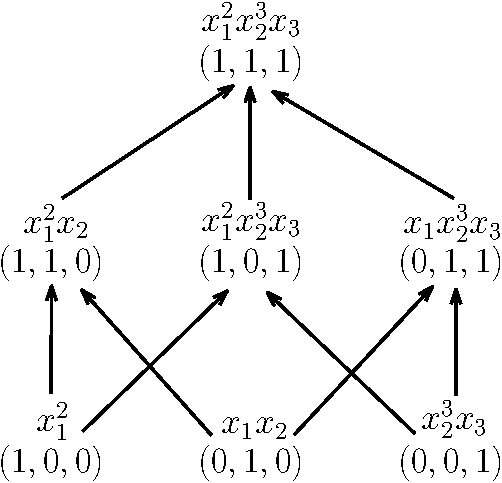
\includegraphics[scale=0.6]{./figures/example_taylor.pdf}
\caption{The simplicial complex associated to the taylor resolution}
\label{fig:taylor}
\end{figure}

In this example, the Taylor resolution is not minimal. In general, the Taylor resolution is far from being minimal.

\end{exmp}

\subsubsection{Scarf Complex}
Unfortunately, the Taylor resolution is usually not minimal. The nonminimality is visible in the nonzero scalars in the differential maps, which occur whenever there exist faces $F$ and $G$ with the same multidegree such that $G$ is in the boundary of $F$. It is tempting to try to simply remove the nonminimality by removing all such faces; the result is the \textit{Scarf complex}.

\textbf{Construction}: Let $I = \langle m_1, \dots, m_r \rangle \subseteq R$ be a monomial ideal. Let $X_{\text{Taylor}}$ be the full simplex on $\lbrace m_1, \dots, m_r \rbrace$, and let $X_{\text{Scarf}}$ be the simplicial subcomplex of $X_{\text{Taylor}}$ consisting of the faces with unique multidegree, $$X_{\text{Scarf}} = \lbrace F \in X_{\text{Taylor}} \vert gr(G) = gr(F) \Longrightarrow G = F \rbrace$$

We say that $X_{\text{Scarf}}$ is the \textit{Scarf simplicial complex} of $I$; the associated algebraic chain complex $\mathbb{F}_{\bullet}^{(X_{\text{Scarf}},gr)}$ is called the \textit{Scarf complex} of I. The multidegrees of the faces of $X_{\text{Scarf}}$ are called the \textit{Scarf multidegrees} of $I$.

\begin{exmp}
Let $I = \langle x_{1}^2, x_{1} x_{2}, x_{2}^3 x_{3} \rangle$. The scarf simplicial complex of $I$ is the complex $X_{\text{Scarf}}$ in figure \ref{fig:scarf}. The scarf complex of $I$ is the minimal resolution $$\mathbb{F}_{\bullet}^{(X_{\text{Scarf}},gr)}: \quad
0 \rightarrow \begin{matrix}
R \lbrack x_{1}x_{2}^{3}x_{3} \rbrack \\ \bigoplus \\
R \lbrack x_{1}^{2}x_{2} \rbrack
\end{matrix}
\xrightarrow{\left( \begin{matrix}
x_{1} & 0 \\
-x_{2}^{2}x_{3} & x_{1} \\
0 & -x_{2}
\end{matrix} \right)}\begin{matrix}
R \lbrack x_{2}^{3}x_{3} \rbrack \\ \bigoplus \\
R \lbrack x_{1}x_{2} \rbrack \\ \bigoplus \\
R \lbrack x_{1}^{2} \rbrack
\end{matrix}
\xrightarrow{\left( \begin{matrix}
x_{2}^{3}x_{3} & x_{1}x_{2} & x_{1}^{2}
\end{matrix} \right)} R/I \rightarrow 0
$$



\begin{figure}[!htb]
\centering
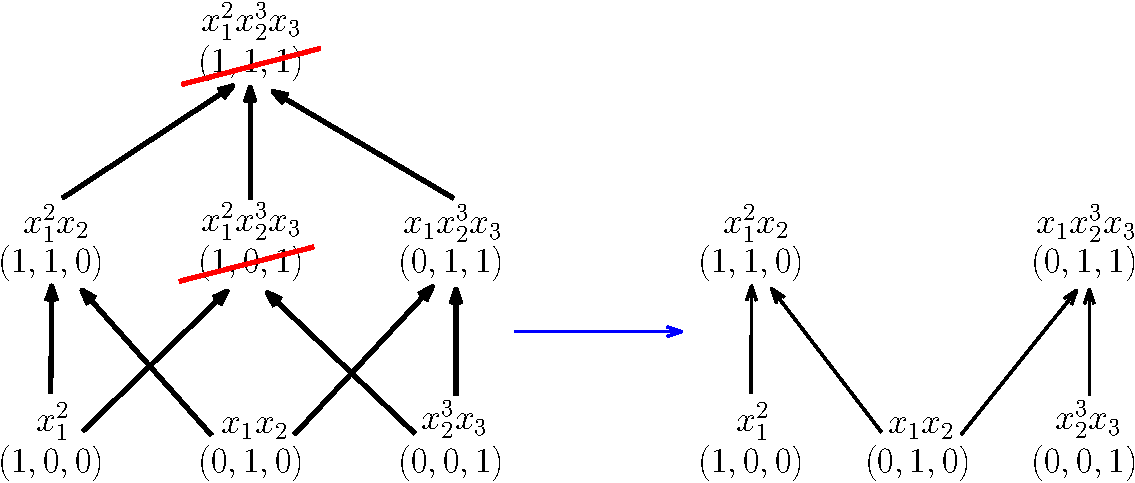
\includegraphics[scale=0.5]{./figures/scarf.pdf}
\caption{The scarf complex obtained from the Taylor resolution}
\label{fig:scarf}
\end{figure}

\end{exmp}

\begin{exmp} \label{ex:scarf not resolution}
$I = \langle x_{1} x_{2}, x_{1} x_{3}, x_{2} x_{3} \rangle = I(C_3)$ the edge ideal of the 3-cycle. The Scarf simplicial complex of $I$ consists of three disjoint vertices. The Scarf complex of $I$ is the complex $$
0 \rightarrow \begin{matrix}
R \lbrack x_{1}x_{3} \rbrack \\ \bigoplus \\
R \lbrack x_{2}x_{3} \rbrack \\ \bigoplus \\
R \lbrack x_{1}x_{2} \rbrack
\end{matrix}
\xrightarrow{\left( \begin{matrix}
x_{1}x_{3} & x_{2}x_{3} & x_{1}x_{2}
\end{matrix} \right)} R/I \rightarrow 0
$$
It is not a resolution
\end{exmp}

Example \ref{ex:scarf not resolution} shows that not every monomial ideal is resolved by its Scarf complex. We say that a monomial ideal is \textit{Scarf} if its Scarf complex is a resolution.

Despite that the Scarf complex is not always a resolution, it is always minimal. It is always a subcomplex of a minimal resolution and when it is a resolution, it is minimal.

\begin{thm} \cite[Theorem 5.5]{Me11}
If the Scarf complex of $I$ is a resolution, then it is minimal.
\end{thm}

\begin{thm} \cite[Theorem 5.6]{Me11}
Let $\mathbb{F}$ be a minimal resolution of $I$. Then the Scarf complex of $I$ is a subcomplex of $\mathbb{F}$.
\end{thm}



\subsubsection{Lyubeznik Resolution}
The Taylor resolution is too large and the Scarf complex is too small. We want to construct simplicial resolutions somewhere in between. There are classes of simplicial resolutions which are in general much smaller than the Taylor resolution, yet still manage to always be resolutions. On such class is the class of Lyubeznik resolutions.

\textbf{Construction}: Let $I = \langle m_1, \dots, m_r \rangle \subseteq R$ be a monomial ideal. Fix an order $m_1 \leq \cdots \leq m_r$  on the generating set of $I$. Consider the simplicial subcomplex $X_{\text{Lyub}} \subseteq X_{\text{Taylor}}$ whose faces of dimension $s$ are labelled by those $\sigma = \epsilon_{i_0} + \cdots + \epsilon_{i_s} \in \lbrace 0,1 \rbrace^r$ such that, for all $t<s$ and all $j<i_t$ $$ m_j \nmid \text{lcm} (m_{i_t}, \dots , m_{i_s})$$

\begin{exmp}
Let $I = \langle x_{1}^2, x_{1} x_{2}, x_{2}^3 x_{3} \rangle$. Independently of the order of the monomials, all faces of dimension 2 will be in the complex, as otherwise it would mean that one of the monomials of the generating set divides another one.

If we fix the ordering $x_{1}^2 \leq x_{1} x_{2} \leq x_{2}^3 x_3$, the Lyubeznik resolution matches the Taylor resolution ($X_{\text{Lyub},1} = X_{\text{Taylor}}$) because $x_{1}^2 \nmid x_{1} x_{2}^3 x_3$. The same happens whith the order  $x_{2}^3 x_3 \leq x_{1}^2 \leq x_{1} x_{2}$ as $x_{2}^3 x_3 \nmid x_{1}^2 x_{2}$. But with the order $x_{1} x_{2} \leq x_{1}^2 \leq x_{2}^3 x_3$ we have $x_{1} x_{2} \mid x_{1}^2 x_{2}^3 x_3$ and so $\sigma = (1,1,1) \notin X_{\text{Lyub},2}$ and $\sigma ' = (0,1,1) \notin X_{\text{Lyub},2}$. With the last order, the Lyubeznik resolution matches the Scarf complex ($X_{\text{Lyub},2} = X_{\text{Scarf}}$).
\end{exmp}

\begin{remk}
It is unclear how to choose a total ordering on the generators of $I$ which produces a smaller Lyubeznik resolution.
\end{remk}

\begin{thm}
The Lyubeznik resolutions of $I$ are resolutions.
\end{thm}

%%%%%%%%%%%%%%%%%%%%%%%%%%%%%%%%%%%%%%%%%%%%%%%%%%%%%%%%%%%%%%%%
\section{Morse Discrete Theory}

We can use the discrete Morse theory as a method to reduce the number of cells in a CW-complex without changing its homotopy type. In \cite{BaWe02} this technique is adapted to the study of cellular resolutions, using the reformulation of discrete Morse theory in terms of acyclic matchings given by Chari in \cite{Ch00} in order to obtain a reduced cellular resolution given a regular one (usually the Taylor resolution).

First, some preliminaries on discrete Morse theory. Consider the directed graph $G_X$ on the set of cells of a regular $\mathbb{Z}^n$-graded CW-complex $(X,gr)$ which edges are given by $$E_X = \lbrace \sigma \longrightarrow \sigma ' \ \vert \ \sigma ' \leq \sigma, \dim \sigma ' = \dim \sigma -1 \rbrace$$
in other words, $\sigma \longrightarrow \sigma '$ is an edge if and only if $\sigma '$ is a facet of $\sigma$.

For a given set of edges $\mathcal{A} \subseteq E_X$, denote by $G_{X}^{\mathcal{A}}$ the graph obtained by reversing the direction of the edges in $\mathcal{A}$, i.e., the directed graph with edges $$E_{X}^{\mathcal{A}} = (E_{X} \setminus \mathcal{A}) \cup \lbrace \sigma' \Longrightarrow \sigma  \ \vert \ \sigma \longrightarrow \sigma ' \in \mathcal{A}\rbrace$$

When each cell of $X$ occurs in at most one edge of $\mathcal{A}$, we say that $\mathcal{A}$ is a \textit{matching} on $X$. A matching $\mathcal{A}$ is \textit{acyclic} if the associated graph $G_{X}^{\mathcal{A}}$ is acyclic. Given an acyclic matching $\mathcal{A}$ on $X$, the $\mathcal{A}$\textit{-critical cells} of $X$ are the cells of $X$ that are not contained in any edge of $\mathcal{A}$. Finally, an acyclic matching $\mathcal{A}$ is \textit{homogeneous} whenever $gr(\sigma) = gr(\sigma ')$ for any edge $\sigma \longrightarrow \sigma ' \in \mathcal{A}$.

\begin{prop} \cite[Proposition 1.2]{BaWe02} \label{prop:matching}
Let $(X,gr)$ be a regular $\mathbb{Z}^n$-graded CW-complex and $\mathcal{A}$ a homogeneous acyclic matching. Then, there is a (not necessarily regular) CW-complex $X_{\mathcal{A}}$ whose $i$-cells are in one-to-one correspondence with the $\mathcal{A}$-critical $i$-cells of $X$, such that $X_{\mathcal{A}}$ is homotopically equivalent to $X$, and that inherits the $\mathbb{Z}^n$-graded structure.
\end{prop}

In the theory of cellular resolutions, we have the following consequence.

\begin{thm} \cite[Theorem 1.3]{BaWe02} \label{thm:matching}
Let $I \subseteq R = k  \lbrack x_1, \dots, x_n \rbrack$ be a monomial ideal. Assume that $(X,gr)$ is a regular $\mathbb{Z}^n$-graded CW-complex that defines a cellular resolution $\mathbb{F}_{\bullet}^{(X,gr)}$ of $R/I$. Then, for a homogeneous acyclic matching $\mathcal{A}$ on $G_X$, the $\mathbb{Z}^n$-graded CW-complex $(X_{\mathcal{A}},gr)$ supports a cellular resolution $\mathbb{F}_{\bullet}^{(X_{\mathcal{A}},gr)}$ of $R/I$.
\end{thm}

Proposition \ref{prop:matching} and theorem \ref{thm:matching} imply that, given a resolution from a CW-complex, if we have an acyclic matching on it, there is another CW-complex whose cells are the cells that are in the matching, and is homotopically equivalent.

The problem is that the CW-complex $(X_{\mathcal{A}},gr)$ that we obtain is not necessarily regular. Therefore, we cannot always iterate the procedure. To overcome this obstacle, we may use \textit{algebraic discrete Morse theory} developed in \cite{JoWe}.

\begin{thebibliography}{9}
\bibitem{BaWe02}
E. Batzies, V. Welker, \textit{Discrete Morse theory for cellular resolutions}. Journal f{\"u}r die reine und angewandte Mathematik \textbf{543} (2002), 147-168.
\bibitem{Ch00}
Manoj K. Chari, \textit{On discrete Morse functions and combinatorial decompositions}. Discrete Mathematics \textbf{217}, (2000).
\bibitem{JoWe}
M. J{\"o}llenbeck, V. Welker, \textit{Minimal Resolutions via Algebraic Discrete Morse Theory}, (2005).
\bibitem{AlFeGi17}
J. \`Alvarez Montaner, O. Fern\'andez-Ramos, Ph. Gimenez, \textit{Pruned cellular free resolutions of monomial ideals}, (2017).
\bibitem{Me11}
J. Mermin, \textit{Three simplicial resolutions}, (2011).
\bibitem{Mo12}
A.M. Bigatti, P. Gimenez, E. S\`aenz-de-Cabez\'on, Eds., \textit{Monomial Ideals, Computations and Applications}, (2012).
\end{thebibliography}
\end{document}